\chapter{
الگوریتم چندشبکه‌ای برای روش عناصر متناهی
}
\label{chp:chap2}\thispagestyle{empty}
پس از مدل‌سازی یک مسئله واقعی به معادله دیفرانسیل نظیر، حل این معادله دیفرانسیل اهمیت پیدا می‌کند.
جواب تحلیلی این معادله دیفرانسیل اهمیت فراوانی دارد اما در بسیاری از مسائل، فرایند پیچیده‌ای دارد که موجب می‌شود در برخی موارد، یافتن این جواب غیرممکن باشد.
بنابراین روش‌های عددی برای دستیابی به جواب تقریبی اهمیت پیدا می‌کنند.
روش‌های عددی مختلفی برای محاسبه تقریبی جواب مسئله وجود دارند که در طول تاریخ توسعه و بهبود یافته‌اند.
یکی از اساسی‌ترین روش‌های عددی،
\eng{FEM}
است.
در ابتدای فصل، ساختار
\eng{FEM}
به‌طور مختصر بیان شده است.
سپس 
\eng{FEM}
با گسسته‌سازی مکانی-زمانی بر مسئله
\eng{SFD}
زیر پیاده‌سازی می‌شود
\begin{equation}
\label{mainEq}
\begin{cases}
\dift{u(x, y, t)} = K_{x} \diffbeta{u(x, y, t)} + K_{y} \diffgamma{u(x,y,t)} + f(x,y,t)
\sqs
(x,y) \in \Omega
\sqs
t \in (0,T]
\sqn
\\
u(x,y,t)=0
\sqs
(x,y) \in \bOmega
\sqs
t \in (0,T]
\sqn
\\
u(x,y,0) = \psi _{0} (x,y)
\sqs
(x,y) \in \Omega
\sqn
\end{cases}
\end{equation}
که در آن
$K_{x}, K_{y} \in \RealP$،
$0.5 < \beta, \gamma < 1$،
$\psi_{0} \in \Lt$
و
$f \in \LtT$.
این پیاده‌سازی به ساخت یک دستگاه برای هر گام زمانی موجب می‌گردد که باید در بعد مکانی حل شود.
از کنار هم قرار دادن دستگاه‌های هر گام زمانی می‌توان یک دستگاه بلوکی ساخت.
این دستگاه در بعد زمانی حل می‌شود و جواب آن، تقریب عددی جواب مسئله
\eqref{mainEq}
در کل نقاط مکانی و زمانی گسسته‌شده است. 
پس از ارائه نحوه ساخت این دستگاه بلوکی و بیان تاریخچه مختصری از روش‌های موازی‌سازی در زمان،
\eng{MGRIT}
معرفی می‌شود که یکی از روش‌های موازی‌سازی در زمان برای حل دستگاه است.
% ==========+==========+==========+==========+==========+==========+==========+==========
\section{
گسسته‌سازی
}
اکنون باید گسسته‌سازی مکانی-زمانی بر فرم ضعیف
\eqref{mainEqWeak}
اعمال شود.
برای راحتی در انجام محاسبات، بهتر است توابعی را به‌عنوان پایه انتخاب کرد که به‌صورت حاصل‌ضربی از یک تابع مکانی در یک تابع زمانی باشند.
بنابراین ابتدا گسسته‌سازی بر روی مکان و سپس گسسته‌سازی بر روی زمان بررسی خواهند شد.
پس از آن، فضاهای لازم برای گسسته‌سازی ترکیبی بیان شده و در فرم ضعیف
\eqref{mainEqWeak}
جایگذاری می‌شوند.
% ==========+==========+==========+==========+==========
\subsection{
گسسته‌سازی مکانی
}
در گسسته‌سازی ناحیه
$\Omega$
از شبکه مثلثی یکنواخت
$\Th$
با ثابت‌های
$\hx = (b-a) / \Mb$
و
$\hy = (d-c) / \Mg$
استفاده شده است.
\begin{figure}[h]
\centering
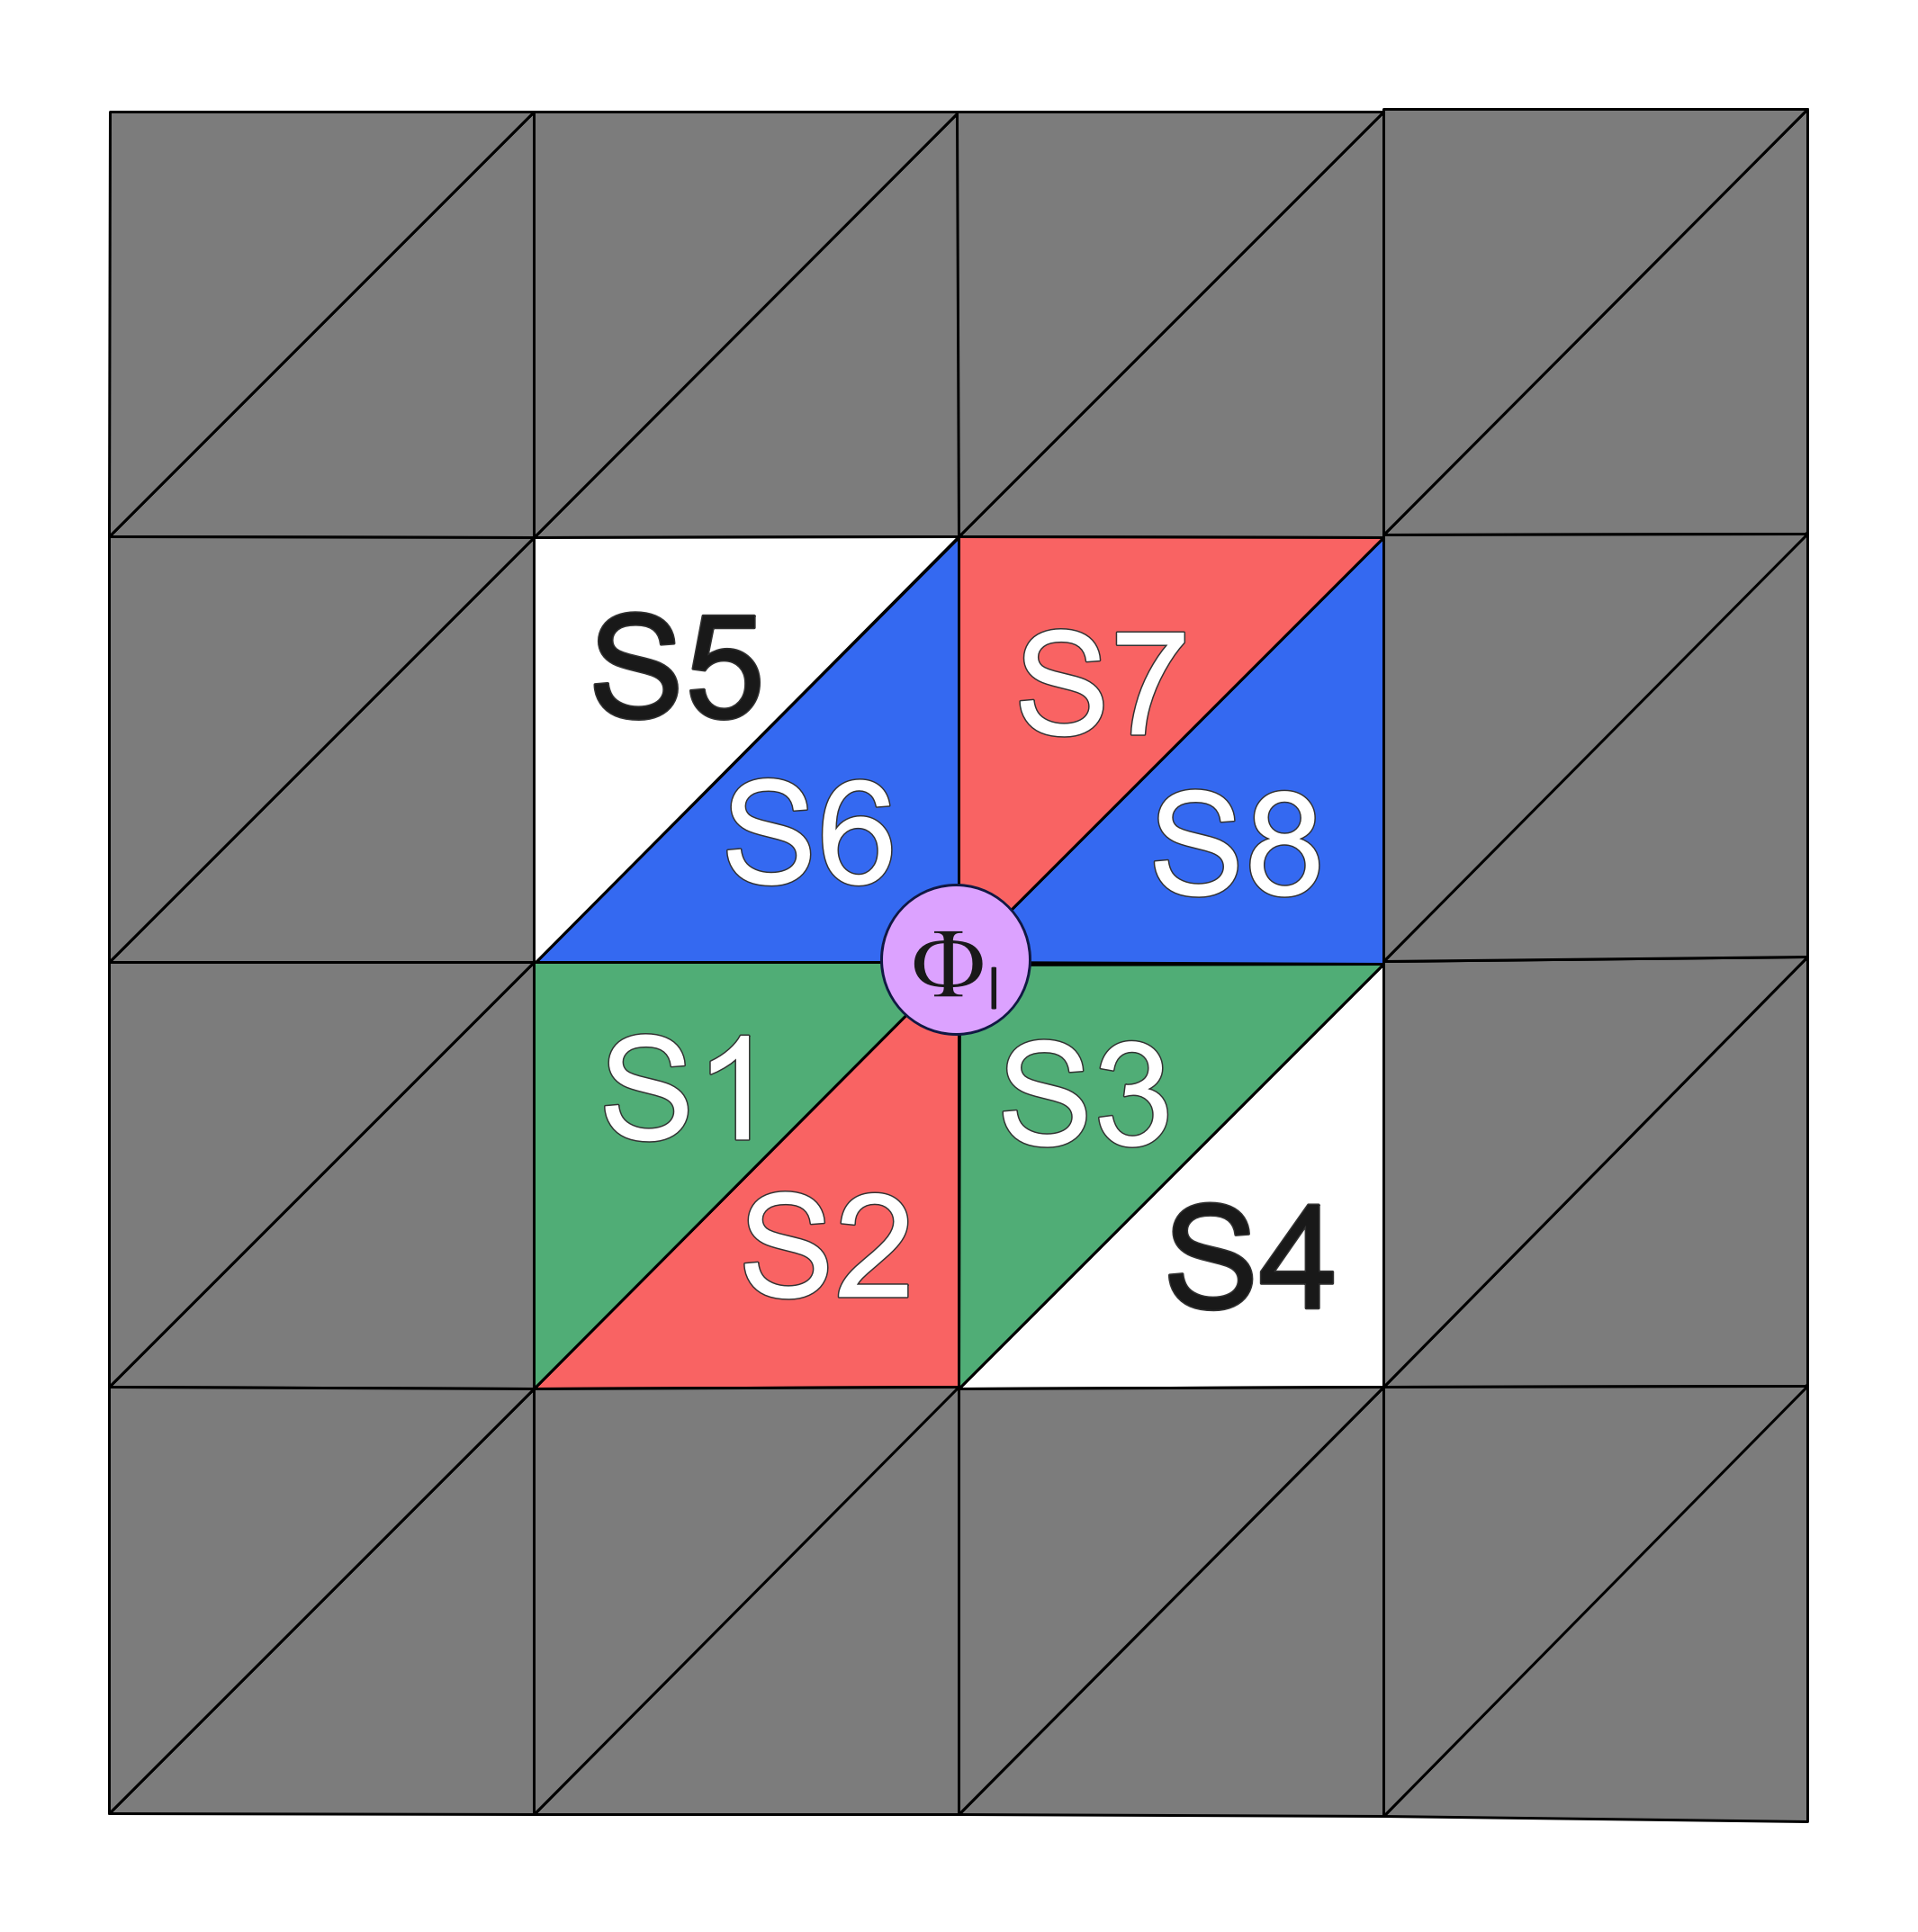
\includegraphics[scale=0.4]{./chapters/chapter2/figures/element.png}
\caption{
عناصر حول یک گره درونی شبکه مکانی.
}
\label{elementFig}
\end{figure}
در شکل
\ref{elementFig}
می‌توان نحوه شبکه‌بندی مثلثی یکنواخت بر بخشی از ناحیه
$\Omega$
را مشاهده کرد.
نحوه شماره‌گذاری عناصر از گوشه سمت چپ پایین ناحیه
$\Omega$
به‌صورت سطری و در راستای محور
$x$
است.

% ==========+==========+==========+==========+==========+==========+==========+==========